\let\negmedspace\undefined
\let\negthickspace\undefined
\documentclass[journal]{IEEEtran}
\usepackage[a5paper, margin=10mm, onecolumn]{geometry}
%\usepackage{lmodern} % Ensure lmodern is loaded for pdflatex
\usepackage{tfrupee} % Include tfrupee package

\setlength{\headheight}{1cm} % Set the height of the header box
\setlength{\headsep}{0mm}     % Set the distance between the header box and the top of the text

\usepackage{gvv-book}
\usepackage{gvv}
\usepackage{cite}
\usepackage{amsmath,amssymb,amsfonts,amsthm}
\usepackage{algorithmic}
\usepackage{graphicx}
\usepackage{textcomp}
\usepackage{xcolor}
\usepackage{txfonts}
\usepackage{listings}
\usepackage{enumitem}
\usepackage{mathtools}
\usepackage{gensymb}
\usepackage{comment}
\usepackage[breaklinks=true]{hyperref}
\usepackage{tkz-euclide} 
\usepackage{listings}
% \usepackage{gvv}                                        
\def\inputGnumericTable{}                                 
\usepackage[latin1]{inputenc}                                
\usepackage{color}                                            
\usepackage{array}                                            
\usepackage{longtable}                                       
\usepackage{calc}                                             
\usepackage{multirow}                                         
\usepackage{hhline}                                           
\usepackage{ifthen}                                           
\usepackage{lscape}
\begin{document}

\bibliographystyle{IEEEtran}
\vspace{3cm}

\title{NCERT-9.3.11}
\author{EE24BTECH11023 - RASAGNA}

% \maketitle
% \newpage
% \bigskip
{\let\newpage\relax\maketitle}

\renewcommand{\thefigure}{\theenumi}
\renewcommand{\thetable}{\theenumi}
\setlength{\intextsep}{10pt} % Space between text and floats


\numberwithin{equation}{enumi}
\numberwithin{figure}{enumi}
\renewcommand{\thetable}{\theenumi}

\textbf{Question:}  
Find the solution of the following differential equation:  
\begin{align*}
    (x + y) \frac{dy}{dx} = 1
\end{align*}
\textbf{Solution:}  
From the question, 
\begin{align}
\frac{dy}{dx}=\frac{1}{x+y}
\end{align}
let,
\begin{align}
    x+y=v
\end{align}
\begin{align}
    \frac{dy}{dx}=\frac{dv}{dx}-1
\end{align}
Substituting into the equation $\brak{0.1}$, we get:
\begin{align}
    \frac{dv}{dx} = \frac{1}{v} + 1
\end{align}
\begin{align}
    \int(1- \frac{1}{1+v})dv = \int{dx}
\end{align}
\begin{align}
v-\ln |1+v|=x+c
\end{align}
putting v=x+y,
\begin{align}
    y-\ln|1+x+y|=c
\end{align}
let us assume  the initial condition to be $y=0$ and $x=1$\\
substituting in equation $\brak{0.7}$,we get the value of c,
\begin{align}
\therefore c={-ln{2}}
\end{align}
the final required equation is,
\begin{align}
    x={2e^{y}-(1+y)}
\end{align}
\textbf{Logic for writing the code(method of finite difference)}
\\
The slope of a tangent at a point $(x_0, y_0)$ on the curve is: 
\begin{align} 
\frac{dy}{dx} = \lim_{h \to 0} \frac{f(x_0 + h) - f(x_0)}{h}
\end{align}
By moving infinitesimally small distance(h) along the tangent , we get another point $(x_1, y_1)$ .the value of $(x_1,y_1)$
\begin{align}
x_1=x_0+h
\end{align}
\begin{align}
y_1=y_0+\frac{dy}{dx}h
\end{align}
Here,
\begin{align}
    \frac{dy}{dx}=\frac{1}{x_0+y_0}
\end{align}
On substituting the value of $\frac{dy}{dx}$ in equation $\brak{0.15}$ we get,
\begin{align}  
y_1=y_0+{\frac{1}{x_0+y_0}}h
\end{align}
Similarly we can obtain n number of points where 
\begin{align}
    x_n=x_{n-1}+h 
\end{align}
\begin{align}
    y_n=y_{n-1}+{\frac{1}{x_{n-1}+y_{n-1}}}h
\end{align}
 Together these points form the curve representing one of the general solutions of the given Differential Equation. The plot is generated by choosing a known point $(x_0, y_0)$ which satisfies the equation.The value of h is taken to be very small.We generate a large number of points and then plot them.
\begin{center}
    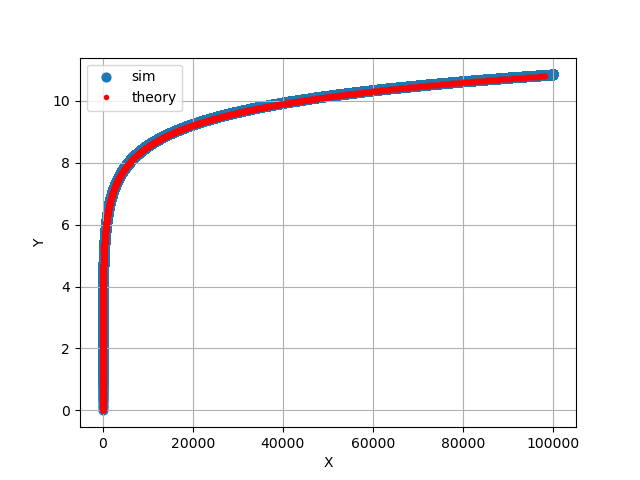
\includegraphics[width=0.75\columnwidth]{figs/fig.png}
\end{center}
\end{document}